
\subsubsection{Análisis para $C_{comp_{2}}$ en modo tensión, $V_{out} = 10 \si[per-mode=symbol]{\volt}$, $R_{L} = 2 \si[per-mode=symbol]{\ohm}$}

Se puede ver en la figura~\figref{fig:fig_power_supply_CCOMP2_LOOP_Modo1} como ya con el valor de $C_{comp_{2}} = 2 \si[per-mode=symbol]{\nano\farad}$ se logra unos márgenes de fase y ganancia aceptables, valores menores o mayores los disminuyen, además seguir aumentando el valor de $C_{comp_{2}}$, solo disminuye innecesariamente el ancho de banda, como se puede ver en la figura~\figref{fig:fig_power_supply_CCOMP2_RF_Modo1}. A nivel de respuesta dinámica no se ven grandes diferencias entre los valores simulados, ver figura~\figref{fig:fig_power_supply_CCOMP2_STEP_0_Modo1}, figura~\figref{fig:fig_power_supply_CCOMP2_STEP_2n_Modo1} y figura~\figref{fig:fig_power_supply_CCOMP2_STEP_5n_Modo1}.

\vfill


% CCOMP2 MODO 1.

\clearpage

\begin{figure}[H] %htb
\begin{center}
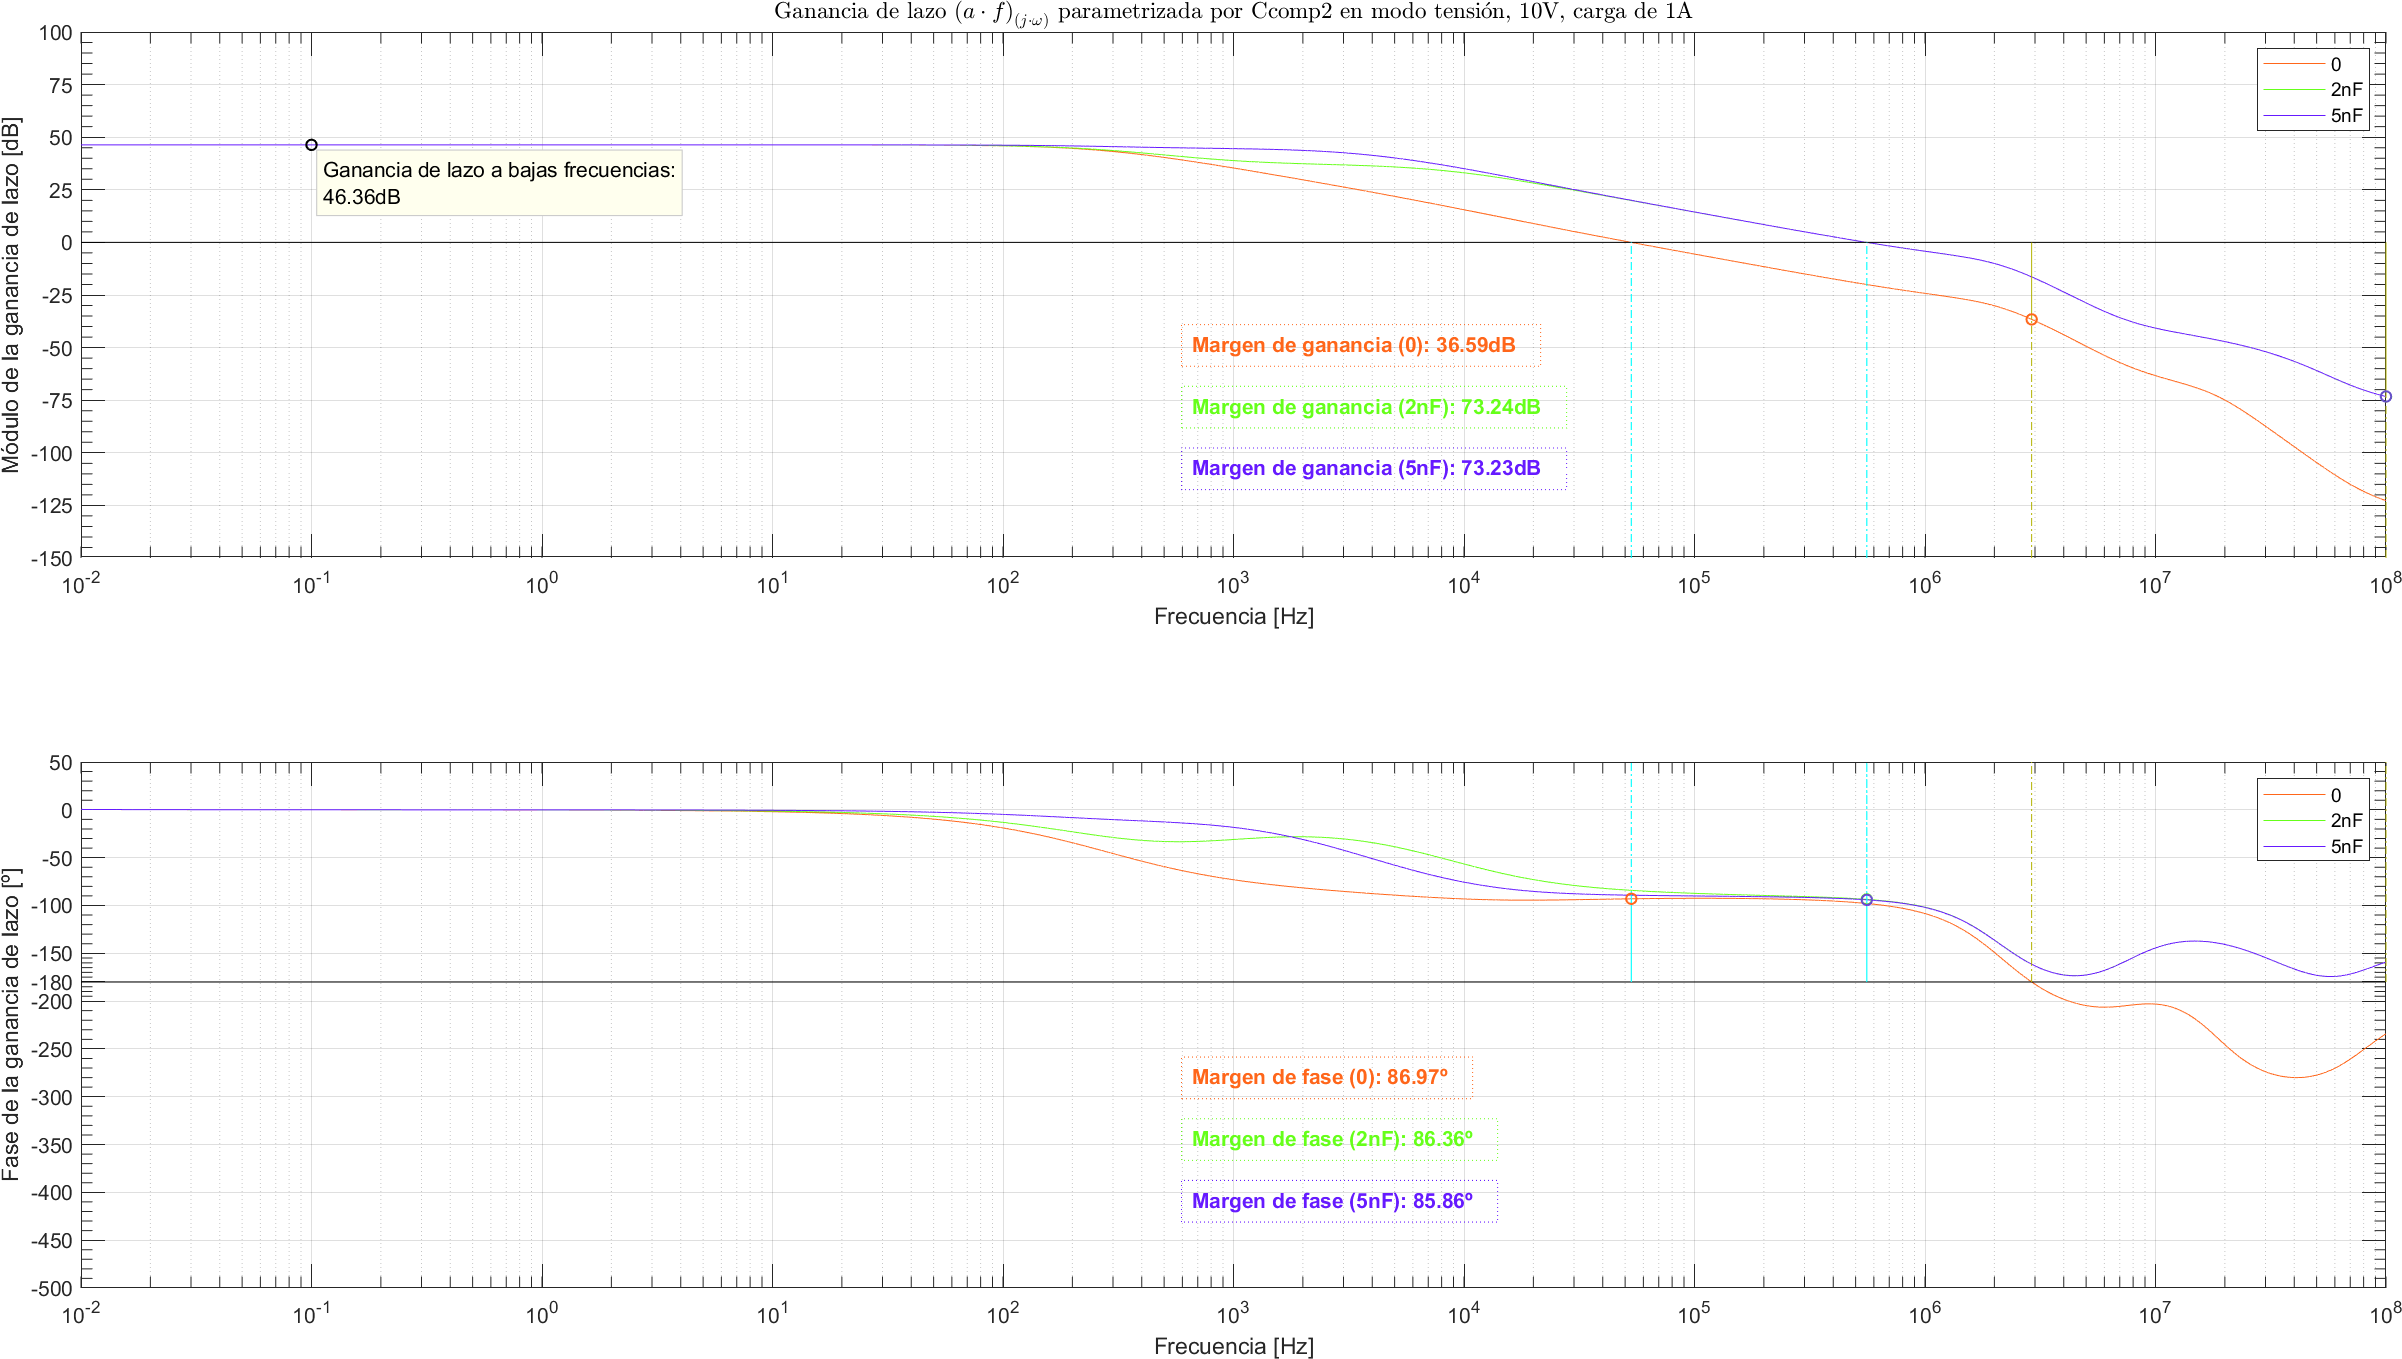
\includegraphics[width=1.1 \textwidth, angle=90]{./img/plots/loop/power_supply_CCOMP2_LOOP_Modo1.png}
\caption{\label{fig:fig_power_supply_CCOMP2_LOOP_Modo1}\footnotesize{Ganancia de lazo en modo tensión, $V_{out} = 10 \si[per-mode=symbol]{\volt}$, en función de la frecuencia parametrizada por $C_{comp_{2}}$.}}
\end{center}
\end{figure}


\clearpage

\begin{figure}[H] %htb
\begin{center}
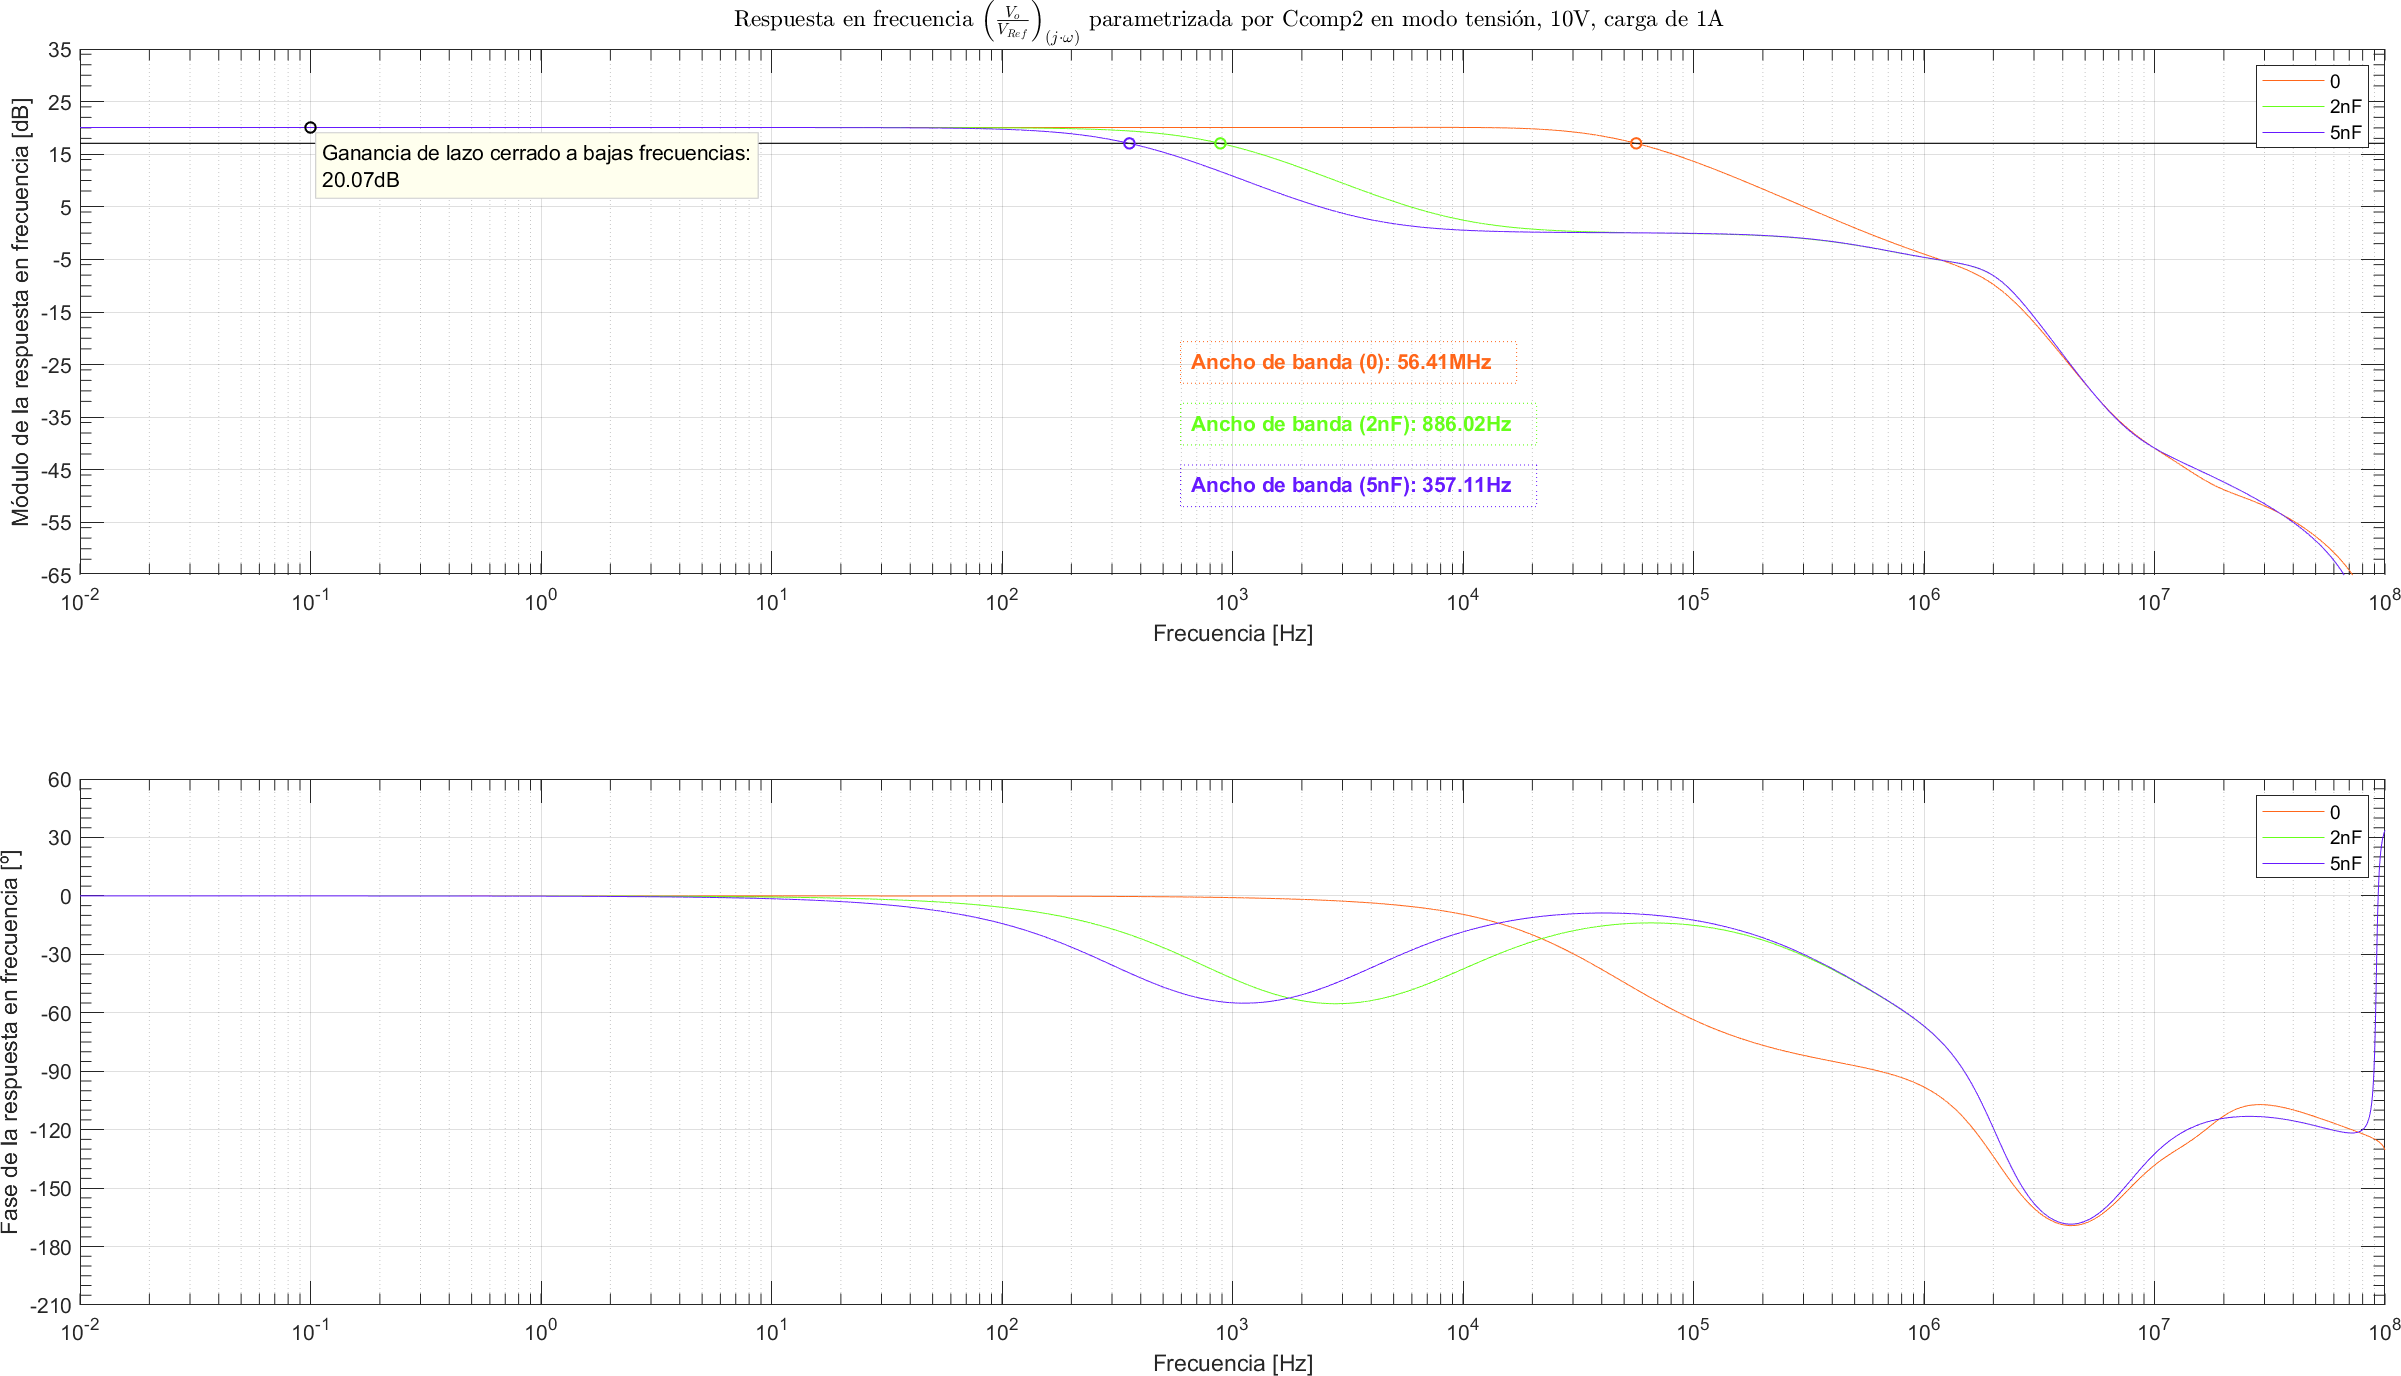
\includegraphics[width=1.1 \textwidth, angle=90]{./img/plots/rf/power_supply_CCOMP2_RF_Modo1.png}
\caption{\label{fig:fig_power_supply_CCOMP2_RF_Modo1}\footnotesize{Respuesta en frecuencia en modo tensión, $V_{out} = 10 \si[per-mode=symbol]{\volt}$, en función de la frecuencia parametrizada por $C_{comp_{2}}$.}}
\end{center}
\end{figure}

\clearpage

\begin{figure}[H] %htb
\begin{center}
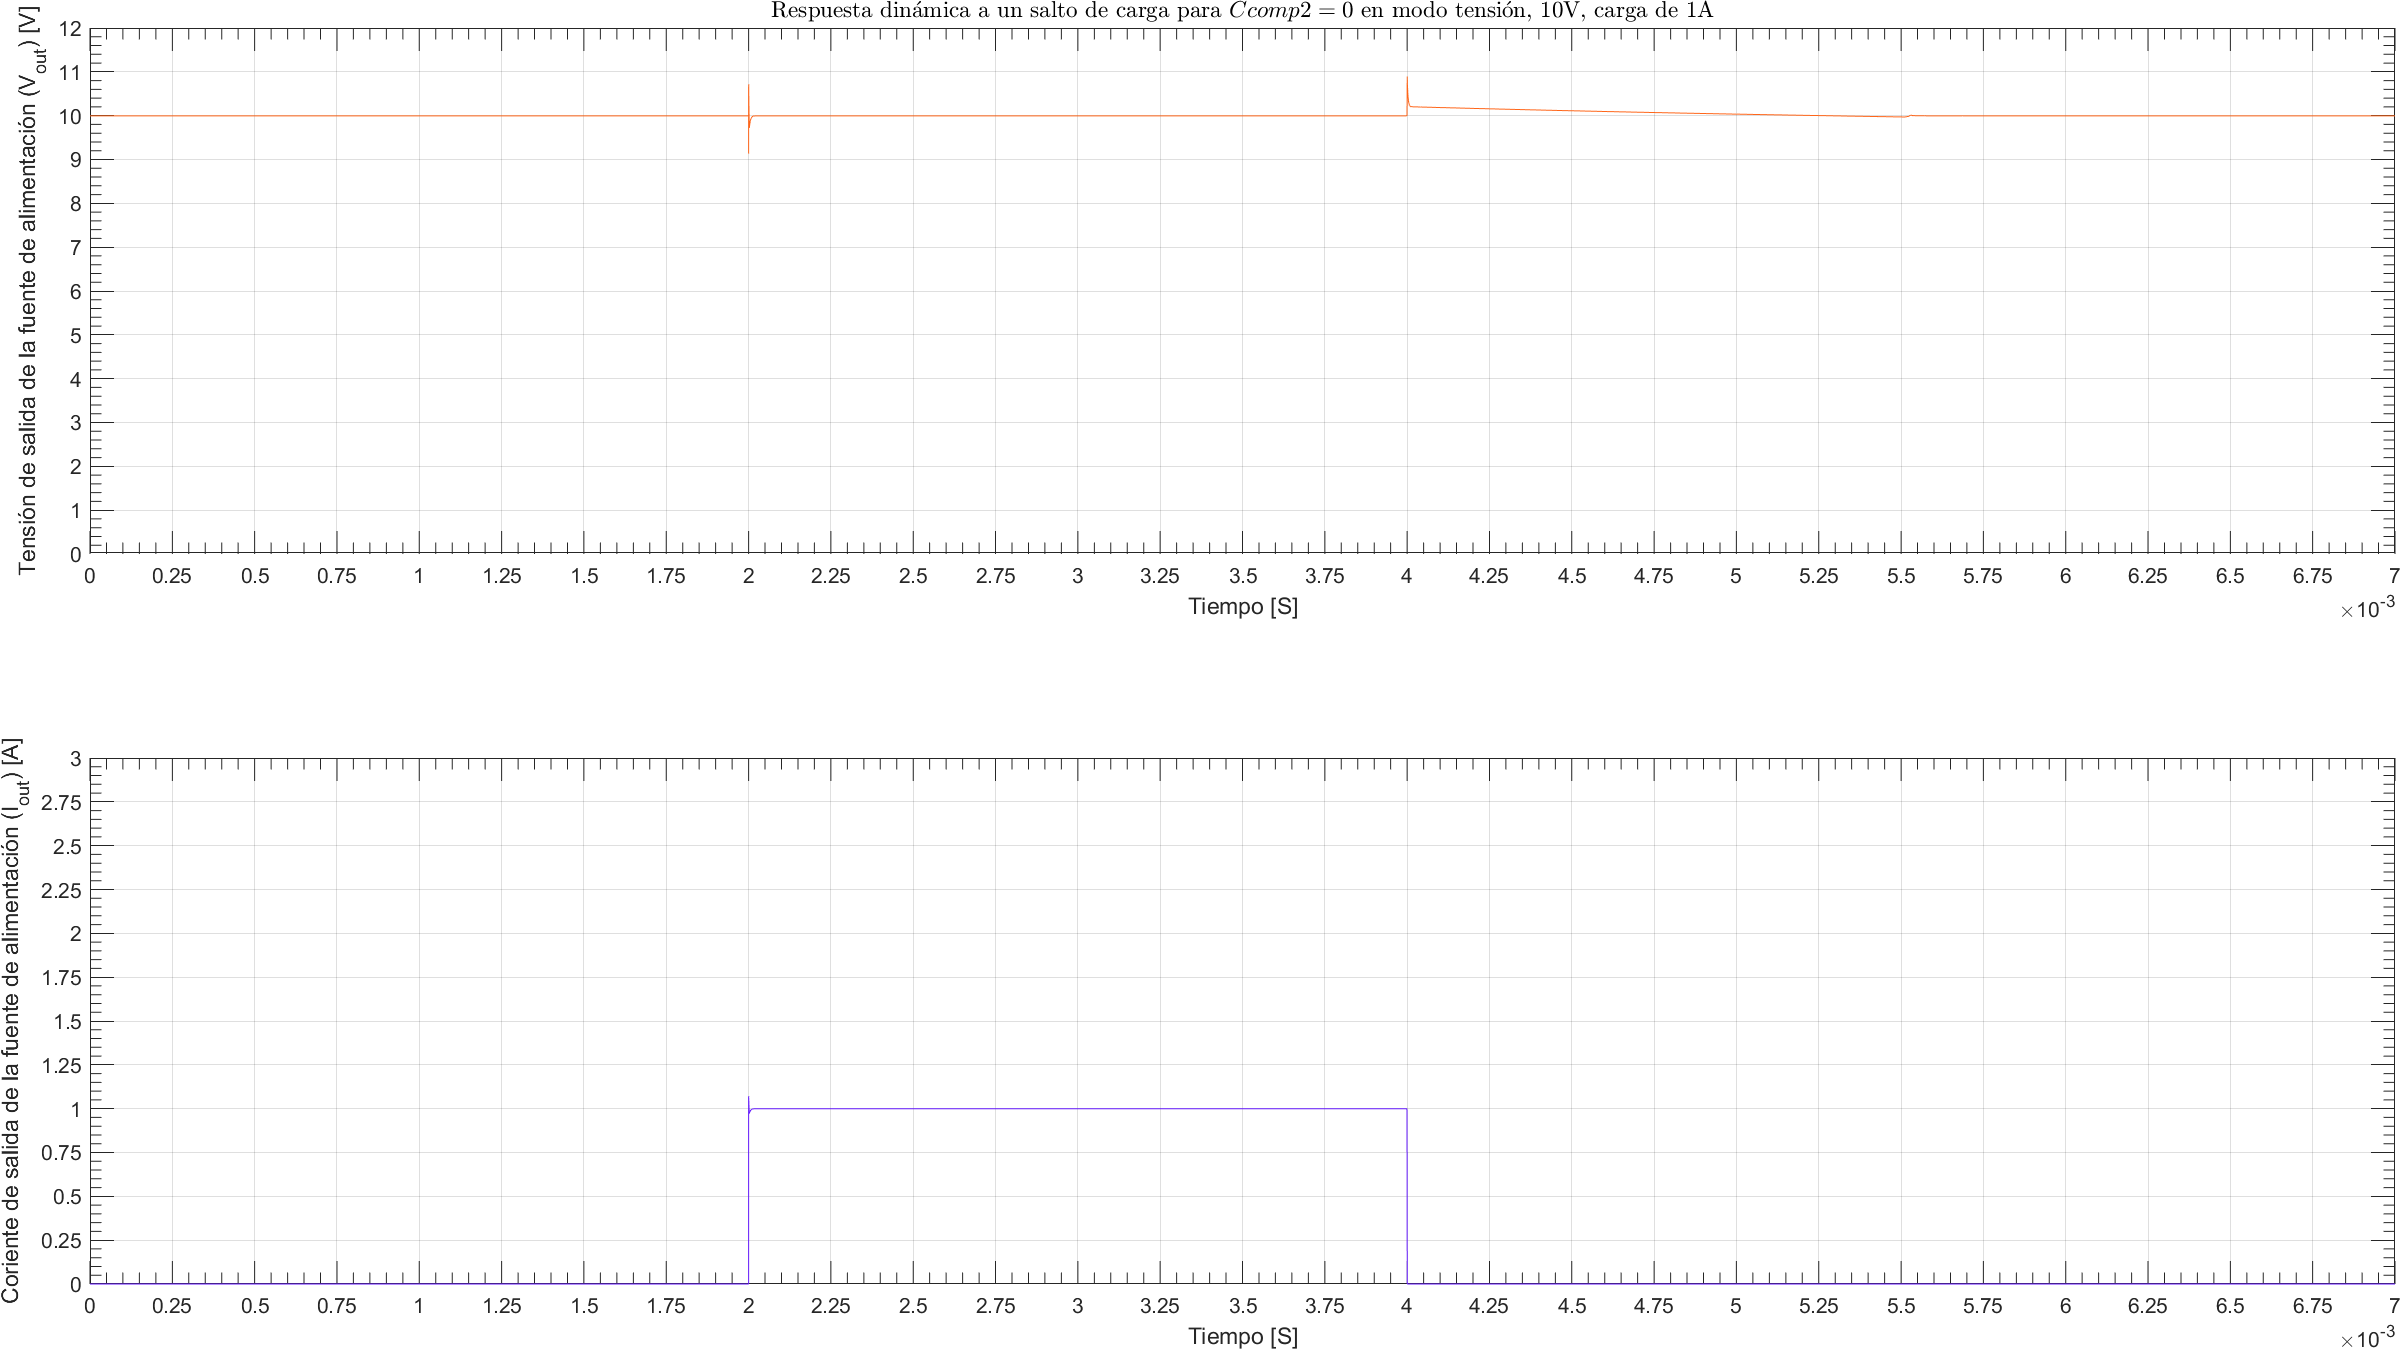
\includegraphics[width=1.1 \textwidth, angle=90]{./img/plots/dynamic/power_supply_CCOMP2_0_STEP_Modo1.png}
\caption{\label{fig:fig_power_supply_CCOMP2_STEP_0_Modo1}\footnotesize{Respuesta dinámica en modo tensión, $V_{out} = 10 \si[per-mode=symbol]{\volt}$, para $C_{comp_{2}} = 0 \si[per-mode=symbol]{\nano\farad} $.}}
\end{center}
\end{figure}

\clearpage

\begin{figure}[H] %htb
\begin{center}
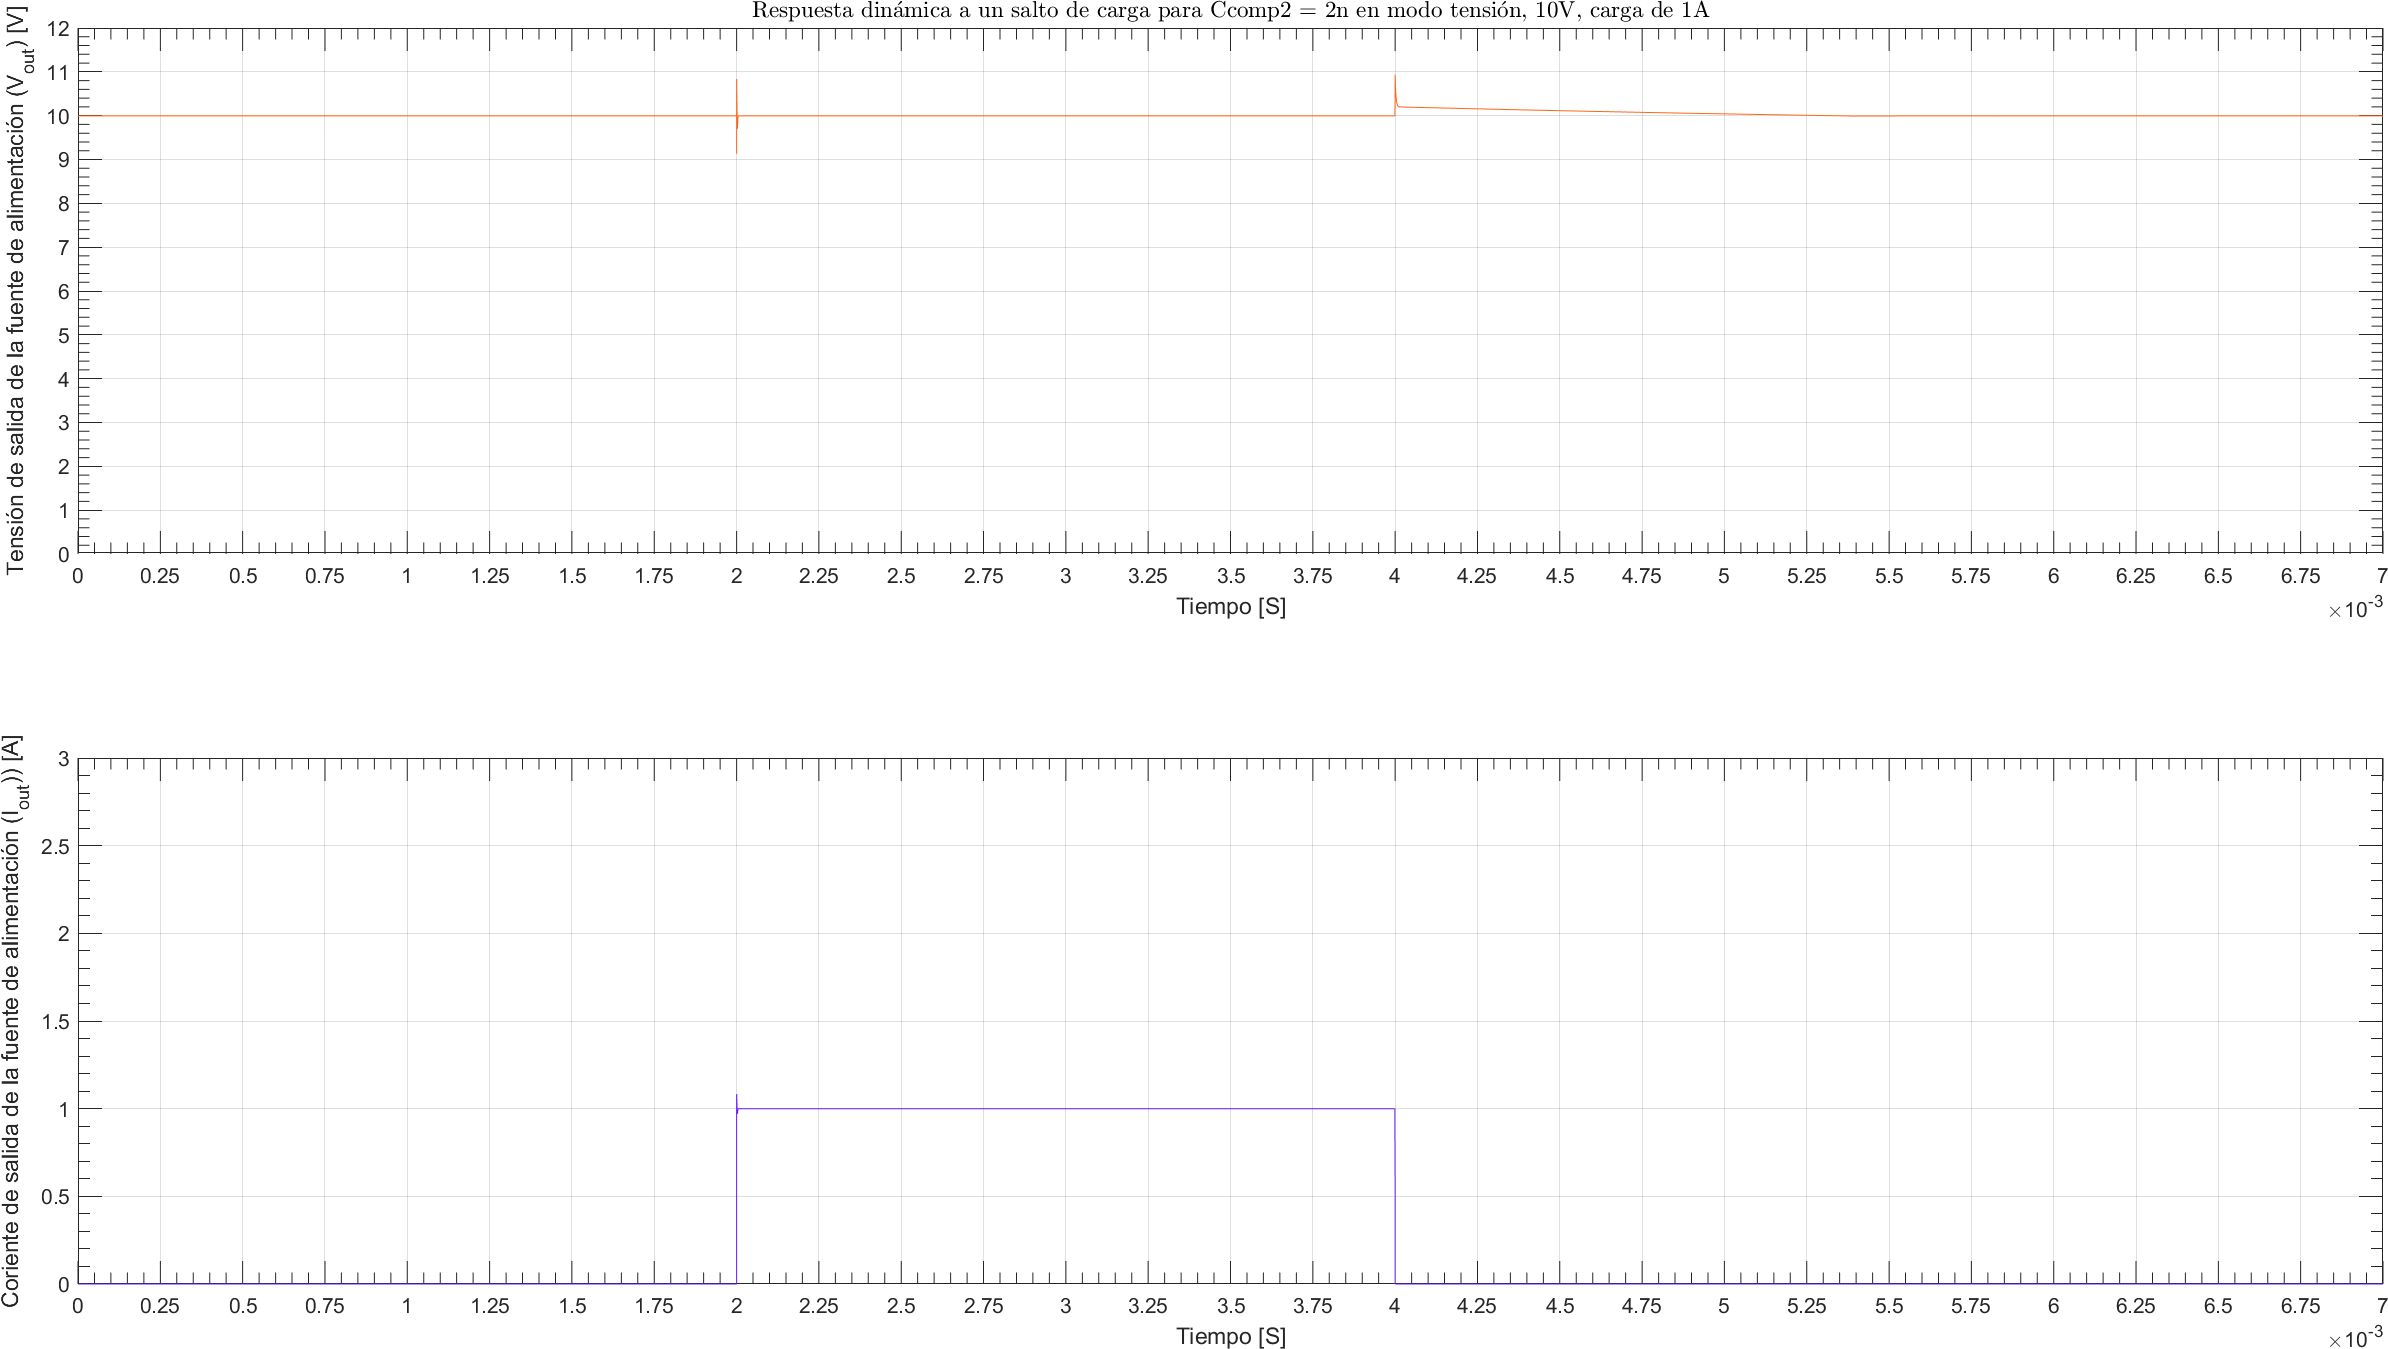
\includegraphics[width=1.1 \textwidth, angle=90]{./img/plots/dynamic/power_supply_CCOMP2_2n_STEP_Modo1.png}
\caption{\label{fig:fig_power_supply_CCOMP2_STEP_2n_Modo1}\footnotesize{Respuesta dinámica en modo tensión, $V_{out} = 10 \si[per-mode=symbol]{\volt}$, para $C_{comp_{2}} = 2 \si[per-mode=symbol]{\nano\farad} $.}}
\end{center}
\end{figure}

\clearpage

\begin{figure}[H] %htb
\begin{center}
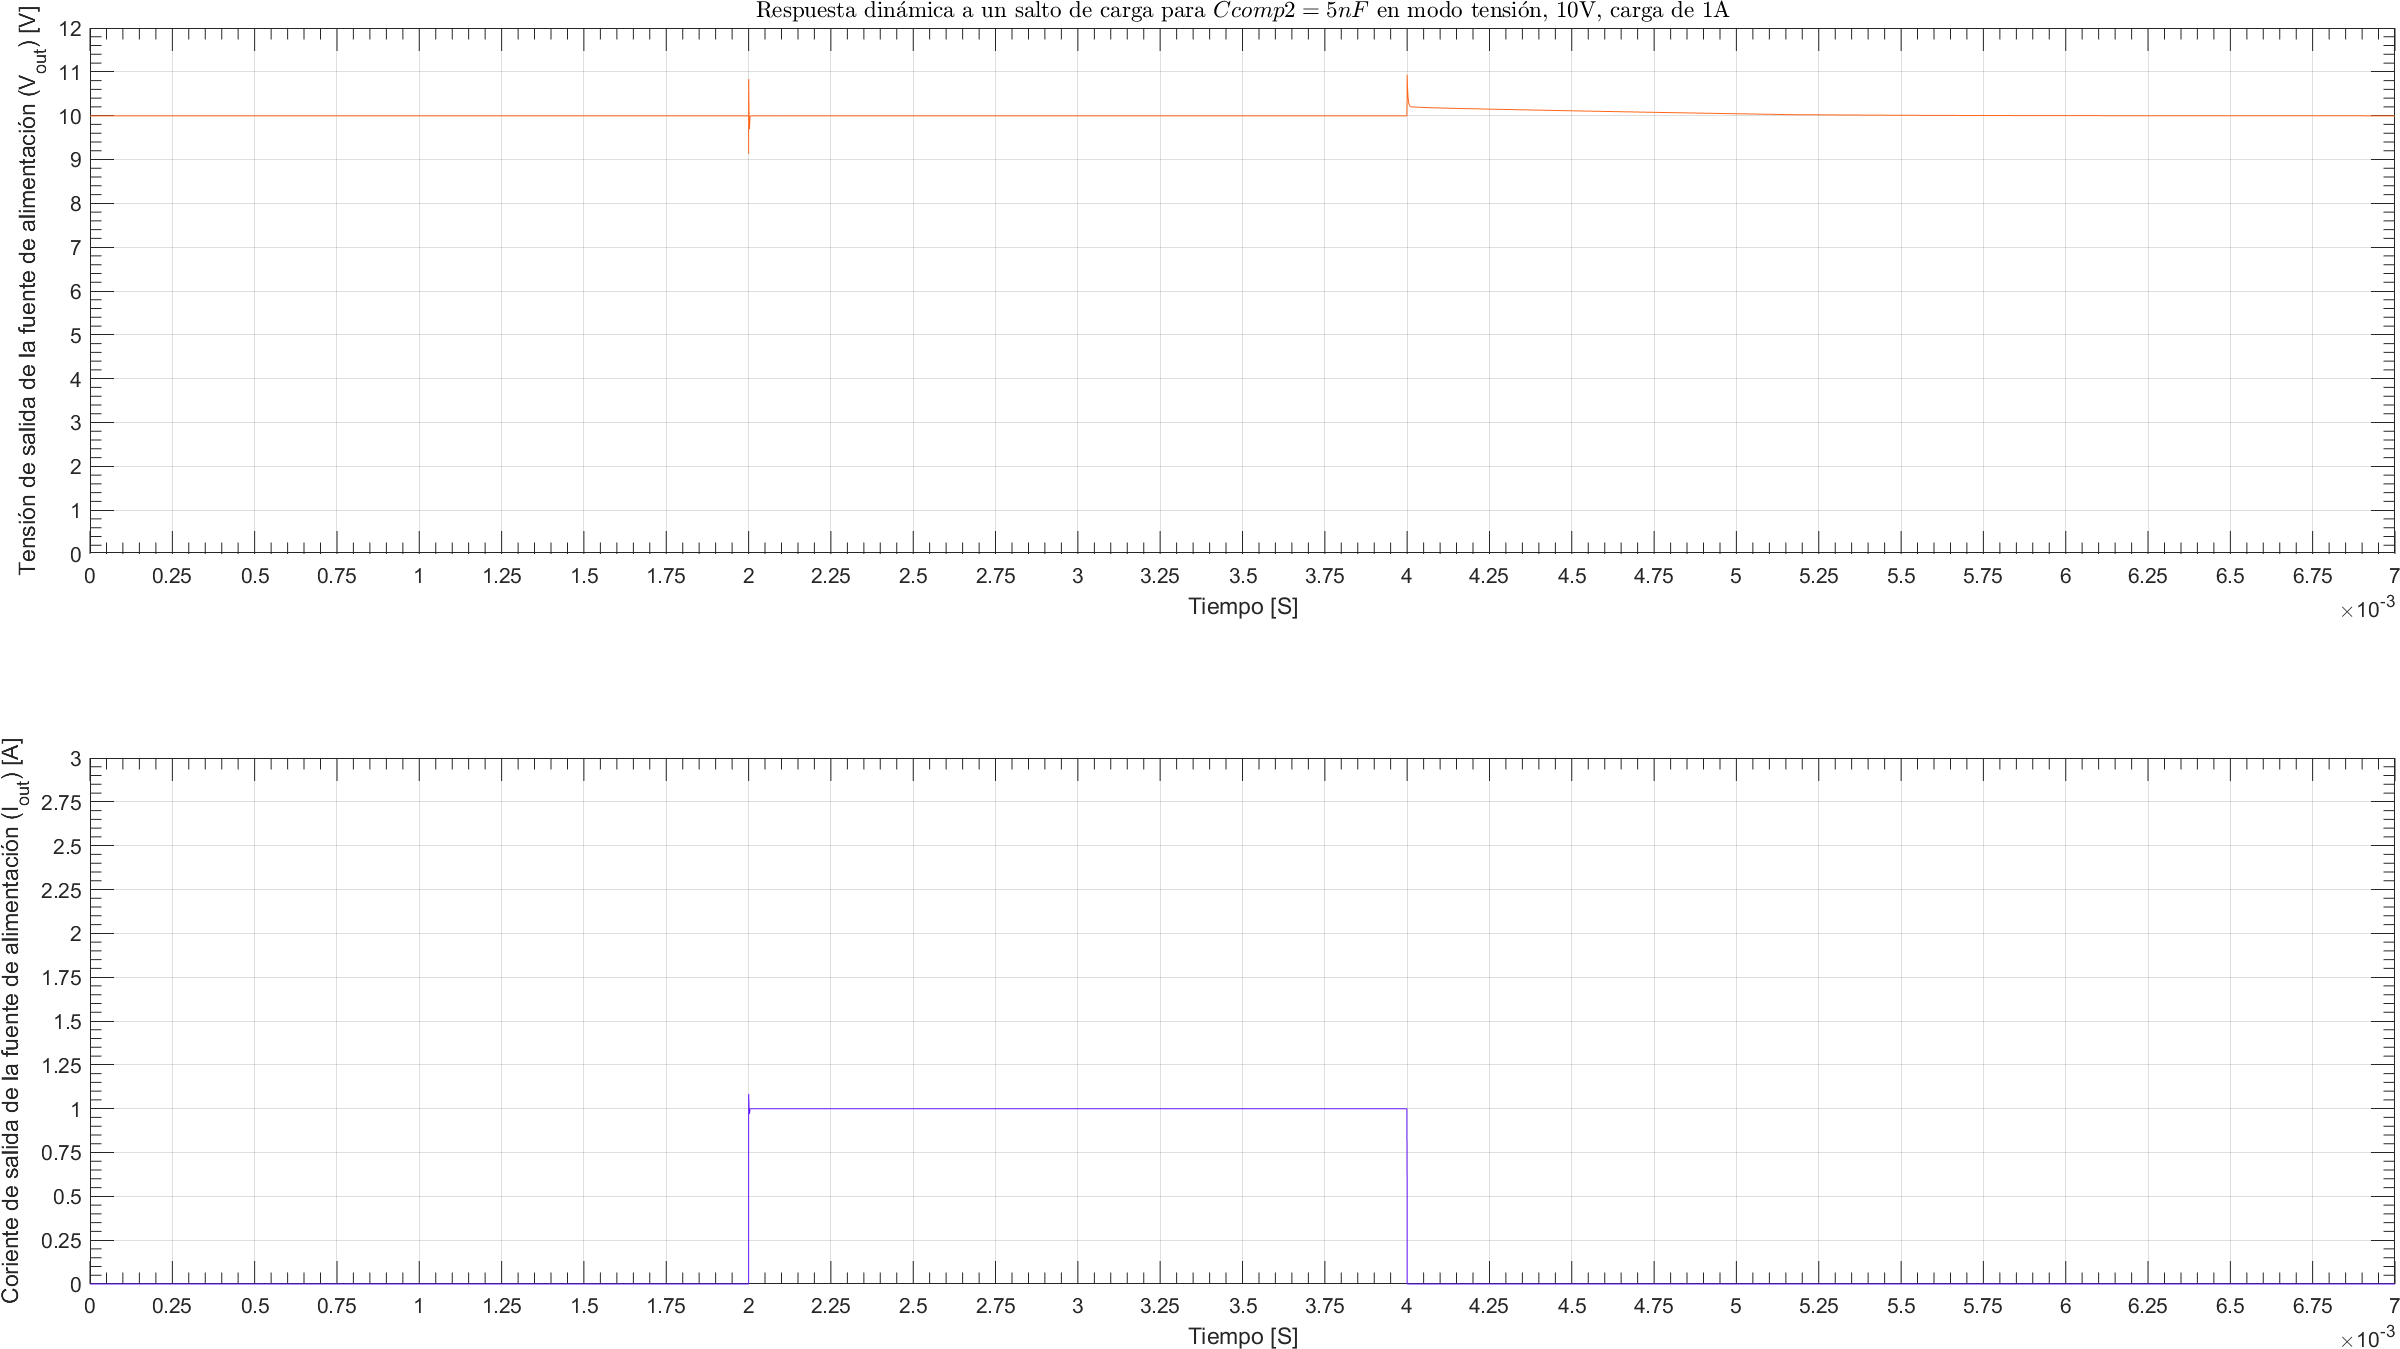
\includegraphics[width=1.1 \textwidth, angle=90]{./img/plots/dynamic/power_supply_CCOMP2_5n_STEP_Modo1.png}
\caption{\label{fig:fig_power_supply_CCOMP2_STEP_5n_Modo1}\footnotesize{Respuesta dinámica en modo tensión, $V_{out} = 10 \si[per-mode=symbol]{\volt}$, para $C_{comp_{2}} = 5 \si[per-mode=symbol]{\nano\farad} $.}}
\end{center}
\end{figure}

\clearpage
